\input{bmsLayoutDoc}


\renewcommand{\author}{Philipp G. Freimann}
\renewcommand{\grafikautor}{Ph. G. Freimann}
\renewcommand{\authoremail}{philipp.freimann@bms-w.ch}
\renewcommand{\erstellungsdatum}{10. Nov. 2021}
\renewcommand{\docversion}{2.36 \TeX}
\renewcommand{\doctitel}{Denksportaufgaben}

\renewcommand{\fachthema}{Mathematischer Denkanstoß---}
\renewcommand{\ausrichtungAufTitelseite}{}

\begin{document}

\ptitlepage
\newpage

\section{Gefangene}\index{Gefangene}
\subsection{Drei Wächter}\index{Wächter}
Ein Verließ\index{Verließ} hat zwei Türen: Die eine führt zur Freiheit\index{Freiheit}, die andere an den
Galgen\index{Galgen}. Dazwischen stehen drei Wächter. Einer, sagt immer die Wahrheit, einer
lügt immer und der Wankelmütige sagt manchmal die Wahrheit, und manchmal
lügt er. Es ist aber nicht bekannt, wer von den Wächtern welche beschriebene
Eigenschaft hat.
Ein Gefangener darf zwei beliebige Fragen stellen, um herauszufinden, wie er in
die Freiheit gelangt. Jede der beiden Fragen darf jedoch nur einer Person
gestellt werden. Natürlich dürfen beide Fragen auch an dieselbe Person gestellt
werden. Es darf aber keine Frage an mehrere Personen gleichzeitig gestellt
werden.
\TNTeop{}


\subsection{Was muss ein Cracker Fragen, um in die Freiheit zu gelangen?}

Nachdem die acht bekanntesten Cracker\index{Cracker} endlich gefangen wurden, konnte
ihnen die Schuld dennoch nicht nachgewiesen werden. \textit{In dubio pro reo} hat
sich der Richter\index{Richter} gesagt und ihnen am Prozesstag den folgenden Vorschlag
gemacht:

\textit{«Ihr werdet in Einzelhaft\index{Einzelhaft} gebracht. Jeder in eine eigene Zelle; in einem
Gefängnis mit acht normalen Zellen und einer speziellen Zelle. Ihr werdet keine
Mittel zur Kommunikation untereinander erhalten. Weder Handy, noch sonst
was. Jeden Tag werde ich jedoch irgendeinen von Euch – ganz zufällig – für eine
Stunde in die spezielle Zelle, die Binärzelle sperren. Darin gibt es lediglich einen
Schalter den ihr vom Zustand 0 auf 1 oder vom Zustand 1 auf 0 umschalten
könnt. Dies ist dann auch die einzige Information\index{Information}, die ihr einander hinterlassen
dürft, bevor am nächsten Tag der nächste (oder nach dem Zufallsprinzip wieder
ihr selbst) in die Binärzelle gebracht wird. Nach einigen Wochen werden dann –
ganz nach meinem Auswahlprinzip – alle Acht von Euch einmal in der Binärzelle
gewesen sein. Viele von Euch aber auch mehrfach! Kann mir einer von Euch nun
den Tag nennen, an dem alle mindestens einmal in der Binärzelle waren, dann
seid ihr alle frei. Ihr dürft mir auch später melden und sagen, dass der besagte
Tag nun definitiv vorbei gewesen sei. Ihr müsst also den exakten Tag nicht
angeben können. Wenn ihr es herausfindet, seid ihr alle frei. Meldet ihr es
jedoch zu früh, wird das Verfahren eingestellt und ihr bleibt für den Rest eures
Lebens hinter Gittern. Morgen beginnt das Verfahren, bis dahin könnt ihr noch
beraten, ob ihr darauf eingehen wollt, oder ob ihr gleich für immer hinter Gitter
wollt.»}

Die Cracker beraten sich und nach einiger Zeit kommen sie zum Schluss, dass
sie diesen Vorschlag annehmen wollen. Was haben sie sich wohl für ein
Verfahren ausgedacht, damit sie sicher freikommen?

\TNTeop{}

\newpage
\TRAINER{%% nur Trainerversion
\subsection{Lösungsvorschlag: Drei Wächter}

Die erste Frage des Gefangenen\index{Gefangene} (an einen beliebigen Wächter) lautet: «Welcher
von Deinen Kollegen lügt seltener?»

\begin{itemize}
\item Gerät der Gefangene an den Wahrheitsliebenden, so zeigt dieser diesem
den Wankelmütigen.
\item Gerät er an den Lügner, zeigt dieser auch den Wankelmütigen.
\item Gerät er an den Wankelmütigen, zeigt dieser auf einen der beiden
anderen.
\end{itemize}

In allen drei Fällen aber ist der, auf den nicht gezeigt wird auch nicht der
Wankelmütige.

Diesem dritten kann man der Gefangene also erfolgreich folgende Frage stellen:
«Welchen Weg in die Freiheit würde mir dein Kollege, der das genaue Gegenteil
von dir ist, zeigen?»

\subsection{Lösungsvorschlag: Cracker}
Die Cracker wählen das folgende Verfahren.
Der erste Cracker, der in die Binärzelle geführt wird, wird zum Senior ernannt.
(Also der am ersten Tag ausgewählte.) Der Senior schaltet \textbf{immer}, wenn er in
die Zelle kommt, den Schalter auf 0. Ab seinem zweiten Tag in der Binärzelle
beginnt er mit dem Zählen. Jedes Mal, wenn er in die Zelle kommt und der
Schalter auf 1 ist, zählt der Senior für sich hoch (und schaltet dann den Schalter
sofort wieder auf 0). Wenn er nun sieben Mal hochzählen konnte, meldet er dem
Richter, dass nun alle Gefangenen mindestens einmal in der Binärzelle waren.

Alle anderen Cracker verfahren wie folgt. Sie dürfen während der ganzen
Gefangenschaft den Schalter in der Binärzellen nur ein einziges Mal von 0 auf 1
umschalten. Kommen sie in die Binärzelle und der Schalter ist bereits auf 1,
dann tun sie gar nichts. Das bedeutet nämlich, dass ein Gefangener vor ihnen
bereits seinen «Zähler» verbraucht hat. Kommen sie jedoch in die Zelle und der
Schalter ist auf 0, so können sie nun den Schalter auf 1 umlegen. Dies dürfen sie
aber, wie erwähnt, während der ganzen Gefangenschaft nur ein einziges Mal
tun. Dieses umlegen zählt nämlich ihren eigenen Besuch in der Binärzelle.

Hat der Senior nun auf 7 gezählt, so ist jeder der anderen Gefangenen bereits
einmal in der Zelle gewesen und der Senior kann dem Richter melden, dass der
Zeitpunkt der Freilassung nun endlich gekommen sei.
Zusatzaufgabe: Programmieren Sie dieses Verfahren, um herauszufinden, wie
lange es im Durchschnitt braucht, bis die acht Cracker frei sind.
}%% END TRAINER Lösungsvorschlag
\newpage


\section{Zwei Eimer}\index{Eimer}
Vor einem Brunnen stehen zwei Eimer. Diese weisen keinerlei Markierungen
auf. Einer der Eimer fasst 5 Liter, der andere fasst 7 Liter. Ziel ist es, einen (1)
Liter abzumessen.

Wie ist vorzugehen? Wer findet die Lösung, bei der am wenigsten umzuschütten
ist?
\TNTeop{}
\TRAINER{%% Lösungsvorschlag nur Trainer}
\subsection{Lösungsvorschlag: Zwei Eimer}

\begin{enumerate}
\item
Beide Eimer leeren.
\item
5 Liter abmessen\index{abmessen} und
\item
in den (leeren) 7-Liter-Eimer füllen.
\item
5 Liter abmessen
\item
und 2 Liter in den 7-Liter-Eimer füllen. Es bleiben 3 Liter im 5-Liter-
Eimer.
\item
7-Liter-Eimer leeren.
\item
Die 3 Liter aus dem 5-Liter-Eimer in den (leeren) 7-Liter-Eimer einfüllen.
\item
5-Liter-Eimer ganz auffüllen.
\item
4 Liter aus dem 5-Liter-Eimer in den 7-Liter-Eimer einfüllen (der ist jetzt
voll); im 5-Liter-Eimer bleibt genau ein Liter übrig.
\end{enumerate}

Andere Variante:
\begin{enumerate}
\item
Beide Eimer leeren.
\item
7 Liter abmessen
\item
in den (leeren) 5-Liter-Eimer füllen. Es bleiben 2 Liter im 7-Liter-Eimer.
\item
5-Liter-Eimer ausleeren.
\item
2 Liter aus dem 7-Liter-Eimer in den 5-Liter-Eimer umfüllen.
\item
7-Liter-Eimer neu füllen.
\item
3 Liter aus dem 7-Liter-Eimer in den 5-Liter-Eimer umfüllen (mehr hat im
5-Liter-Eimer nicht Platz).
\item
5-Liter-Eimer ausleeren.
\item
Die 4 verbleibenden Liter aus dem 7-Liter-Eimer in den 5-Liter-Eimer
einfüllen.
\item
7-Liter-Eimer wieder auffüllen.
\item
Ein Liter aus dem 7-Liter-Eimer in den 5-Liter-Eimer einfüllen (es bleiben
6 Liter im 7-Liter-Eimer).
\item 
5-Liter-Eimer entleeren.
\item
5 Liter aus dem 7-Liter-Eimer in den 5-Liter-Eimer füllen. Es bleibt ein
Liter im 7-Liter-Eimer.
\end{enumerate}

}%% END TRAINER
\newpage
\section{Zahlen}\index{Zahl}  
\subsection{Französischer Spion}\index{Spion}\index{französischer Spion}
Im Deutsch-Französischen Krieg\index{Krieg} 1870/71 will ein französischer Spion
unbemerkt in eine deutsche Stadt gelangen. Die Stadt hat eine Schutzmauer
und wird von einem Wächter bewacht. Der Franzose versteckt sich in einem
Gebüsch und versucht herauszufinden, wie die Stadtbewohner an der Wache
vorbeikommen.

Zuerst kommt ein Bauer\index{Bauer} und der Wächter ruft fragend «8 . Der Bauer antwortet
«4» und wird hineingelassen. Jetzt kommt eine Nonne und wird vom Wächter
gefragt: «16»? Sie antwortet «8» und wird ebenfalls eingelassen. Jetzt kommt ein
Mönch. Der Wächter fragt nach «28». Der Mönch antwortet «14». Auch er kann
passieren.

Jetzt glaubt unser Französische Spion das Spiel durchschaut zu haben und geht
auf das Stadttor\index{Stadttor} zu. Er wird vom Wächter nach «14» gefragt, antwortet mit «7»
und wird noch am selben Tage exekutiert.

Was hätte er auf die Frage des Wächters antworten sollen?

\subsection{Falsche Rechnungen?}\index{Rechnungen!falsche}
In dieselbe Kategorie geht die Aufgabe, die mir ein Kursteilnehmer per E-Mail
zur Verfügung gestellt hat.

8890 = 6

6633 = 2

7722 = 0 

7563 = 1

7387 = 2

1838 = 4

7237 = 0
 
5656 = 2

8398 = 5

1386 = ???

\TNTeop{}

\TRAINER{%%
\subsection{Lösungsvorschlag: Spion}
Die Zahlen sind als Text zu lesen und nicht als Zahlenwerte oder Ziffernfolge.
Die Zahl „acht“ hat 4 Buchstaben.

„Sechzehn“ hat 8 Buchstaben.

„Achtundzwanzig“ hat 14 Buchstaben.

Somit hätte der Spion auf die Frage „14“ einfach 8 antworten sollen.

\subsection{Lösungsvorschlag: Falsche Rechnungen}

Zählen Sie einfach die Anzahl der geschlossenen Kreise\index{Kreis}. 6, 9 und 0 besitzen je
einen Kreis, 8 besitzt 2 Kreise. (Die Aufgabe kann am besten von
Vorschulkindern gelöst werden.)

Lösung 1386 = 3
}%% END TRAINER

\newpage

\section{Wiegeprobleme}\index{Wiegeprobleme}
\subsection{König}\index{König!Wiegeprobleme}



Der König treibt im ganzen Land die Steuern ein. Jeder der 100 Bürger muss
einen Sack mit 1000 Goldmünzen\index{Goldmünzen} abliefern. Dem König wird bekannt, dass unter
den Bürgern ein Betrüger ist, dessen Goldmünzen gefälscht sind. Seine Münzen
sind rein optisch von den anderen nicht zu unterscheiden, wiegen aber nur 9g,
anstelle der gewöhnlichen 10g.

Wie kann der König mit nur einem
Wiegevorgang den Betrüger\index{Betrüger} herausfinden?

Bemerkung: Der König hat eine sehr
genaue Waage, die jedoch nur ein einziges Mal funktioniert.

\TNTeop{}

\subsection{Karamell}\index{Karamell}\index{Krämer}
Der Besitzer eines Krämerladens möchte Zucker pfundweise von einem bis zu
40 Pfund abwiegen\index{abwiegen} können. Er hat nur eine altmodische Waage zur Verfügung,
bei der die abzuwiegende Menge in einer Waagschale mit den entsprechenden
Gewichten in der anderen Schale ausbalanciert wird. Da er ein effizienter und
sparsamer Mann ist, will er sich nur so viele Gewichte besorgen, wie unbedingt
nötig sind, um jede Menge von einem bis zu 40 Pfund in einem einzigen
Wiegevorgang abzuwiegen.

a) Wie viele Gewichte\index{Gewichte} benötigt er und wie groß sind sie, wenn sie nur auf einer
Seite der Waage benutzt werden dürfen?

b) Wie viele Gewichte sind nur noch nötig, wenn er Gewichte auf beide Schalen
legen darf?
\TNTeop{}

\TRAINER{%%
\subsection{Lösungsvorschlag: König}

Der König nimmt vom ersten Sack 1 Münze, vom zweiten Sack 2 Münzen, vom
dritten Sack 3 Münzen, usw. heraus. Bei 100 Säcken hat er 5050 Münzen
herausgenommen, die somit (unterstellt keine sei gefälscht) 50.500g wiegen
müssten. Beträgt sein Wiegeergebnis allerdings beispielsweise 34g weniger, so
weiß er, dass der Bürger, dem er 34 Münzen aus dem Sack genommen hat der
Betrüger ist! Denn seine Münzen sind ja 1g leichter.

Quelle: \texttt{www.denksport-ecke.de}


\subsection{Lösungsvorschlag: Karamell}

(Quelle: Paul Sloane: Neue Denkpuzzles für helle Köpfe):
Tipp: Ob Sie’s glauben oder nicht, es ist tatsächlich möglich, jedes beliebige
Gewicht zwischen einem und 40 Pfund mit nur vier verschiedenen Gewichten
abzuwiegen. Das setzt allerdings voraus, dass es erlaubt ist, die Gewichte in
beide Waagschalen zu legen (Aufgabe b). Wenn Sie nur eine Waagschale für die
Gewichte benutzen dürfen (Aufgabe a), dann brauchen Sie insgesamt 6
Gewichte. Doch damit können Sie dann alle Gewichte von einem bis 63 Pfund
bestimmen.

a) Die Gewichte haben die Massen 1, 2, 2, 5, 10 und 20 Pfund. Alternativ: 1, 2,
4, 8, 16 und 32 Pfund. Vorteil der 1. Variante: Gängige Zahlen sind einfacher zu
berechnen. Vorteil 2. Variante: Sogar Gewichte bis zu 63 Pfund sind alle
abmessbar.

b) Die Massen betragen: 1, 3, 9 und 27 Pfund.
Um Beispielsweise 16 Pfund abzuwiegen, legt der Kramer 28 (27 + 1) Pfund auf
die eine Schale und 12 (9 + 3) Pfund auf die andere Schale: 28 – 12 ergibt 16
Pfund: so braucht er nur noch 16 Pfund Zucker auf die zweite Schale zu kippen
und die Waage ist im Gleichgewicht.
}%% END TRAINER
\newpage

\section{Prozentrechnungen}\index{Prozentrechnungen}


\begin{center}\textit{«125\% der Leute können nicht Bruchrechnen. Das ist jeder vierte, nein mehr
noch: jeder fünfte!»}\end{center}


\subsection{Skonto}\index{Skonto}

Beim Kauf\index{Kauf} ab zwei Artikeln\index{Artikel} gewährt der Verkäufer 5\% Rabatt\index{Rabatt}. Bei einer
Barzahlung\index{Barzahlung} gewährt er zusätzlich 3\% Skonto. Ist es nun schlauer, das Skonto
zuerst einzufordern und dann die 5\% Rabatt oder besser zuerst die 5\% Rabatt
und dann die 3\% Skonto?

\TNTeop{}

\subsection{Gemüse}\index{Gemüse}
Ein Früchte- und Gemüsehändler hatte eine Tonne (1000kg) Gemüse (z. B.
Gurken\index{Gurken}) geerntet. Seine Messung hatte ergeben, dass die Ware zu 98\%\,
(Gewichtsprozente) aus Wasser besteht.
Leider konnte er das Gemüse auf dem Markt nicht sofort verkaufen, sodass es
einige Tage liegen blieb. Als er es endlich verkaufen kann, ergibt die Messung,
dass die Ware nur noch einen Wasseranteil von 95\% aufweist.
Wie schwer ist die Ware nun?

\TNTeop{}

\subsection{Umsatzsteigerung}\index{Umsatz}
Ein Händler gibt neu einen Rabatt von 10\% auf sein Sortiment. Laut
Branchenverband müsste der Händler nun 70\% mehr Umsatz\footnote{Umsatz = Einnahmen durch Verkauf der Ware, also Einkaufspreis + Marge.} 1 machen, wie vor
der Reduktion, um den ursprünglichen Gewinn zu erzielen.
Reichen diese Angaben, um die ursprüngliche Marge\footnote{Marge = Differenz von Einkaufspreis zum Verkaufspreis; m. a. W. der gesuchte
Gewinn.} 2 zu bestimmen?

\TNT{12}{}\newpage


\TRAINER{%%
\subsection{Lösungsvorschlag: Skonto}

Die Reihenfolge spielt keine Rolle, es sei denn, es werde zwischen den beiden
Abzügen auf- oder abgerundet. Begründung: 5\% Rabatt entspricht einer
Multiplikation mit Faktor 0.95; 3\% Skonto entspricht einem Faktor 0.97. Nun
gilt aber
(Preis * 0.95) * 0.97 = (Preis * 0.97) * 0.95 (Kommutativgesetz) = 0.9515
Noch besser wäre es, vom Verkäufer direkt 8\% einzufordern, sofern er damit
einverstanden wäre ;-)

5.5. Lösungsvorschlag: Prozentrechnung
Der einfachste Weg geht hier über den festen Bestandteil des Gemüses. Die
erste Messung ergibt einen Wasseranteil von 98\%, das bedeutet, dass das
Gemüse anfänglich einen Anteil von 980kg Wasser enthält: lediglich 20kg sind
kein Wasser (also fester Bestandteil).
Die zweite Messung ergibt einen Wasseranteil von 95\%. Das bedeutet aber, dass
5\% fester Anteil sind. 5\% sind aber die 20kg aus der ersten Messung. Die
Festbestandteile haben sich ja nicht geändert. Nun lautet die Aufgabe viel
einfacher: 20kg entsprechen 5\%, wie viel sind 100%?
Die einfache aber doch noch etwas verblüffende Antwort lautet: 400kg (wovon
380kg Wasser sind.)
Man könnte sich nun fragen: „Was(?), eine Abnahme von 3\% Wasser macht
600kg aus?“ Das wäre natürlich falsch. Es werden ja eben nicht einfach 3\% des
Wassers entzogen, sondern das Verhältnis Wasser zu Festbestandteil ändert
sich um 3\%.
\newpage

\subsection{Lösungsvorschlag: Umsatzsteigerung}

\textbf{Zeitpunkt 1 (vor dem Abschlag):}

Einkaufspreis Ware vorher = EP1 = 100% = 1 (z. B. 100.- CHF)
$$m = \text{(Aufschlags)Marge (als Faktor) vor dem Abschlag}$$
$$\text{Verkaufspreis ursprünglich} = EP \cdot{} (1+m) = 1+m,$$
da ich EP auf eine Einheit (EP) gesetzt hatte (\zB $100.- \cdot{} (1+m)$)


\textbf{Zeitpunkt 2 (nach dem Abschlag, aber vor der Umsatzsteigerung):}

$(1+m)\cdot{}0.9$ = Verkaufspreis nach dem Abschlag (vor der Umsatzsteigerung)

$y := (1+m)\cdot{}0.9 - 1 =$ Marge nach der Reduktion (als Faktor z. B. 0.15 o. ä.)

\textbf{Zeitpunkt 3 (nach der Umsatzsteigerung gegenüber Zeitpunkt 1):}

$1.7(1+m)$ = Umsatzsteigerung gegenüber ursprünglichem Umsatz


$x :=$ Zunahme im Einkauf (unbekannt) (als Faktor gegenüber dem ursprünglichen Einkaufspreis)

$xy =$ Gewinnzunahme gegenüber dem Gewinn aus Zeitpunkt 2.

$1+x = $neuer Einkauf (genau $EP \cdot{} (1+x)$)

$1+y + x + xy =$ neuer Umsatz (Genau genommen $EP \cdot{} (1+y) + x\cdot{}EP \cdot{}(1+y)$,
daher das $xy$)

$y+xy = $neuer Gewinn (und dieser muss ja gleich der alten Marge sein $(y+xy=m)$)
Der neue Umsatz muss nun gleich 170\% des ursprünglichen Umsatzes sein.

Ergo:

$$\Longrightarrow 1+x+y+xy = 1.7(1+m)$$

Die drei Gleichungen nun so (1:1) in \texttt{wolframalpha.com} eintragen:

wolframalpha.com -> $$\{ y=9*(1+m)/10-1, y+xy=m, 1+x+y+xy=17*(1+m)/10\}$$

(die 2. Lösung $m=-1$, also die Marge = -100\% vor der Reduktion ist hier zu
vernachlässigen, das würde bedeuten, er habe die Ware immer gratis
abgegeben.)

Frei nach Wolframalpha:

* Ursprüngliche (Aufschlags)Marge: \textbf{17/63}

* Neue (Aufschlags)Marge: 1/7

* Einkaufszuname: 8/9

PS: Natürlich müssen wir die Resultate an einem Zahlenbeispiel noch
nachrechnen; also eine Probe machen, ob die Resultate sinnvoll sind.
Das Gleichungssystem nicht von Hand ausrechnen: a) geht zu lange b) ist
fehleranfällig.
\newpage
}%% end TRAINER


\section{Alter}\index{Alter}
\subsection{Petra und Anton}\index{Petra und Anton}\index{Anton und Petra}

Petra ist jetzt 24 Jahre alt. Sie ist doppelt so alt wie Anton war, als Petra so alt
war, wie Anton jetzt ist.

Wie alt ist Anton?


\subsection{Du und ich}\index{Du und ich}

Als du so alt warst wie ich heute bin, warst du dreimal so alt wie ich. Und wenn
ich dreimal so alt sein werde wie ich heute bin, dann sind wir zusammen genau
ein Jahrhundert alt.

Wie alt bin ich? Wie alt bist Du?


\subsection{Aus einer Mathematikolympiade (Singapur)}\index{Mathematikolympiade}
Alice und Bob haben Zegna kennen gelernt und wollen ihren Geburtstag wissen.
Zegna nennt den beiden zehn mögliche Daten:

15. Mai, 16. Mai, 19. Mai,

17. Juni, 18. Juni,

14. Juli, 16. Juli,

14. August, 15. August und 17. August.


Zegna\index{Zegna} verrät Alice nur den Geburtsmonat und Bob nur den Tag. Dann sprechen
die beiden miteinander.

Alice sagt zu Bob: «Ich weiß nicht, wann Zegna Geburtstag hat, aber ich weiß,
dass Du es auch nicht weißt.»

Darauf erwidert Bob: «Zu Anfang wusste ich auch nicht, wann Zegna Geburtstag
hat, aber jetzt, dank Deiner Information\index{Information}, weiß ich es.»

Alice: «Jetzt kenne ich ihren Geburtstag auch.»

Wann hat Zegna Geburtstag?
\TNTeop{}


\subsection{Wo ist der Vater?}

Die Mutter ist um 21 Jahre älter als ihr Kind. In sechs Jahren wird dann die
Mutter fünf mal so alt sein wie das Kind. Wo ist der Vater jetzt?

\TNTeop{}

\TRAINER{
\subsection{Lösungsvorschlag: Anton und Petra}

Anton ist 18. Damals in der Vergangenheit, war er halb so alt, also 12 Jahre.
Petra war aber damals gleich alt, wie Anton heute ist:

\begin{tabular}{|c|c|c|}\hline
                      & Petra & Anton\\\hline
 Vergangenheit (war)  & $x$   & 12 \\\hline
 Gegenwart (ist)      & 24    & $x$\\\hline
 \end{tabular}

Die Differenz von $x$ bis 24 muss aber gleich groß sein, wie die Differenz von 12
zu $x$.

In Formeln: $24-x = x - 12$ woraus folgt, dass $x = 18$.
 

\subsection{Lösungsvorschlag: Ich und Du}

Wieder kann die Lösung mit einer Tabelle einfach gefunden werden:

\begin{tabular}{|c|c|c|}\hline
 & du &  ich \\\hline
war (Vergangenheit) & $3x$ & $x$ \\\hline
ist (Gegenwart) & $5x$ & $3x$  \\\hline
sein wird (Zukunft) & $11x$ & $9x$\\\hline
 \end{tabular}
 
11X + 9X = 100 woraus folgt, dass X = 5 ist. \textbf{«Ich bin 15, du bist 25»}

\newpage

\subsection{Lösungsvorschlag: Mathematikolympiade}

\begin{tabular}{|c|c|c|c|c|c|c|}\hline
       & 14. & 15. & 16. & 17. & 18. & 19.\\\hline

Mai    &     & 1.  & 1.     &     &     & 1. \\\hline
Juni   &     &     &        & 1.  & 1.  &  \\\hline
Juli   &  2. &     & Lösung &     &     & \\ \hline
August & 2.  & 2.  &        & 3.  &     & \\\hline
 \end{tabular}

1.: Mai und Juni fallen weg, ansonsten wüsste Alice nicht, ob es Bob weiß (18.
Juni und 19. Mai wären eindeutig für Bob).

2.: Nun weiß es Bob, somit fällt der 14. weg.

3.: Da es Alice schlussendlich weiß, fällt der August weg.


\subsection{Lösungsvorschlag: Wo ist der Vater?}

Nach dem Lösen der Gleichung [$(x+21)+6 = 5\cdot{}(x+6)$; $x$ = Alter des Kindes
heute] erhalten wir, dass das Kind heute genau $-\frac34$ Jahre, also minus neun
Monate alt ist.

}%% END Trainer
\newpage


\section{Hüte}\index{Hüte}
\subsection{Zwerge in der Grotte}\index{Zwerge}\index{Grotte}
In einer stockfinsteren Grotte sind 10 Zwerge von einer bösen Hexe eingesperrt
worden. Jeder hat im Dunkeln einen roten oder grünen Hut erhalten. Die
Zwerge werden aufgefordert, die Hüte anzuziehen und einzeln aus der Grotte
ins Licht zu treten. Sie können die Farbe ihres eigenen Hutes nicht sehen.
Weiter werden sie angewiesen, mit niemandem zu kommunizieren und sich in
einer Reihe aufzustellen.

Wenn sie es nun schaffen, sich so in einer Reihe nebeneinander aufzustellen,
dass alle Zwerge mit grünen Hüten auf der einen Seite stehen und alle mit roten
Hüten auf der anderen Seite, dann werden sie freigelassen.
Wie stellen es die Zwerge an?


\subsection{Fünf Hüte}
\textbf{Drei} Philosophen\index{Philosophen} werden von Indianern gefangen genommen. Doch der
Häuptling gewährt Gnade, wenn die Philosophen ein Rätsel lösen können. Dabei
werden die drei in dunkle Zelte gebracht, wo jeder einen Hut erhält.

Es hat insgesamt \textbf{zwei rote}\index{rot!Hut} und \textbf{drei blaue}\index{blau!Hut} Hüte.

Die Philosophen können die Farbe ihres eigenen Hutes nicht sehen und werden
gleichzeitig auf den Platz geführt. Das Rätsel besteht nun darin, dass die
Philosophen die Farbe ihrer eigenen Hüte erraten sollten.

Kurz vor Ablauf der Bedenkzeit erraten die Philosophen alle gleichzeitig ihre
Hutfarbe. Wie haben sie es geschafft? Was ging in ihrem Denkprozess vor?
Tipp: Philosophen sind gründliche Denker. Da sie im Denken alle auch geübt
sind, denken alle etwa gleich rasch und kommen daher auch beinahe
gleichzeitig auf die Hutfarbe.

\TNTeop{}


\TRAINER{

\subsection{Lösungsvorschlag: Zwerge}
Der erste und der zweite Zwerg haben keine Probleme. Sie stellen sich einfach
nebeneinander. Der dritte Zwerg kann jetzt (dank dem Licht) die beiden Hüte
der bereits „aufgereihten“ Zwerge sehen.

Haben alle Zwerge in der Reihe dieselbe Farbe auf, so stellt er sich an den
Reihenanfang oder ans Reihenende. Hat es jedoch bereits verschiedene Farben,
so drängt er sich zwischen rot und grün hinein. Egal, welche Farbe er selbst
trägt, die Bedingung mit der sortierten Reihe ist dann immer noch erfüllt.

So kann nun jeder der folgenden Zwerge vorgehen.

\subsection{Lösungsvorschlag: Philosophen}
Gehen wir davon aus, dass sie alle etwa gleich schnell überlegen, dann ist das
Problem lösbar. Wir unterscheiden drei Fälle:

1. Wären zwei rote Hüte im Spiel, so würde derjenige mit dem blauen Hut
sofort rufen «ich habe Blau» und daher wüssten auch die beiden
Anderen, dass sie selbst nichts Anderes als rote Hüte aufhaben könnten.

2. Wäre nur ein roter Hut im Spiel, so dauerte der Überlegungsprozess doch
etwas länger: Jeder der beiden «Blauhüte» merkt, dass er selbst nicht rot
sein kann, denn sonst würde der andere «Blauhut» sofort losschreien. Der
«Rothut» kann hier jedoch direkt jedoch noch nichts herausfinden und
schweigt besser eine Weile. Somit wird nach einer kurzen Weile (aber
nicht sofort) einer der «Blauhüte» seine Farbe erraten und der «Rothut»
merkt, dass er selbst es nicht erraten konnte; somit muss er der «Rothut»
sein.

3. Wenn nun aber alle einen blauen Hut bekommen, wird es vertrackter.
Jetzt kann keiner der drei Philosophen seine Farbe direkt erraten; alle
befinden sich nun nämlich in der Situation des «Rothutes» aus dem 2.
Fall. Doch da weder sofort, noch nach kurzer Bedenkzeit das Rätsel gelöst
wurde, bleibt nur noch dieser letzte Fall übrig (drei rote Hüte hatte es ja
nicht zur Auswahl); und somit können auch in diesem Fall (jedoch nach
einiger Überlegung) die drei Philosophen das Rätsel lösen und jeder ruft
kurz vor Ablauf der Bedenkzeit: «Ich trage einen blauen Hut!»

}%% end TRAINER


\newpage


\section{Kamele}\index{Kamele}
\bbwCenterGraphic{4cm}{kamel.png}
\subsection{Bierkrüge}\index{Bierkrüge}

Der Landmann will die Intelligenz des Städters testen. Dazu fragt er letzteren:

«Wie alt sind meine Kamele? Ich habe drei, und das Produkt (Multiplikation)
ihrer Alter beträgt 36 Jahre.»

«Keine Ahnung», antwortet der Städter: «Das ist eindeutig zu wenig
Information\index{Information}.»

Der Landmann: «Nun gut, so bilde denn die Summe der drei Alter, und Du
erhältst die Zahl meiner Bierkrüge im Keller.»

Der Städter geht in den Keller des Bauern, und zählt geduldig die Krüge. Als er
den letzten Krug gezählt hat, bemerkt er: «Das reicht aber immer noch nicht.»

«Noch eins: das älteste Kamel ist mindestens 2 Jahre älter als jedes der beiden
anderen», fügt der Bauer als letzte Information an. Jetzt kennt der
Städter das Alter der Kamele.

Und Du?
\TNTeop{}


\subsection{Das Erbe}\index{Erbe}
Ein reicher Araber\index{Araber} stirbt und hinterlässt seinen drei Söhnen eine Kamelherde
von 17 Kamelen. Noch bevor sich die Kinder über das Erbe streiten können,
finden sie das Testament mit folgender Aufteilung:

Dem ersten Sohn vermache ich die Hälfte der Herde.

Der zweite Sohn erbt einen Drittel der Herde.

Der jüngste Sohn schließlich erhält noch einen Neuntel der Herde.

Die Söhne sind nahe am Verzweifeln, wie die Herde aufzuteilen sei, da kommt
ein Weiser auf einem Kamel geritten und hört sich die Geschichte an. Nach
kurzem überlegen schenkt er den drei Erben sein Kamel und legt sich unter eine
Palme zum Mittagsschlaf.

Als er wieder aufwacht, bedanken sich die drei Söhne bei ihm für die Hilfe,
geben ihm Wasser und Datteln mit auf den Weg und lassen den Weisen auf
seinem Kamel weiterziehen.

Was ist geschehen?

\TNTeop{}

\TRAINER{
\subsection{Lösungsvorschlag: Bierkrüge}

Das Rätsel: wichtig ist, dass dem Städter die Summe auch noch nichts sagt. Hier
alle Möglichkeiten:

\begin{itemize}
\item
 36 = 36 * 1 * 1 Summe: 38

\item
 36 = 18 * 2 * 1 Summe: 21

\item
 36 = 12 * 3 * 1 Summe: 16

\item
 36 = 9 * 4 * 1 Summe: 15

\item
 36 = 9 * 2 * 2 Summe: 13

\item
 36 = 6 * 6 * 1 Summe: 13

\item
 36 = 6 * 3 * 2 Summe: 11

\item
 36 = 4 * 3 * 3 Summe: 10
\end{itemize}

Das heißt, es ist eine der Lösungen (9+2+2) oder (6+6+1). Da es genau ein
ältestes Kamel hat, ist es 9 Jahre alt. Lösung: (9 Jahre, 2 Jahre und
2 Jahre).

\subsection{Lösungsvorschlag: Erbe}
Nachdem die Herde mit dem Kamel des Weisen auf 18 Kamele angestiegen ist,
ist die Aufteilung nach dem Testament möglich.

Der erste Sohn erhält 9 (=1/2), der nächste 6 (=1/3) und der jüngste 2 (=1/9)
Kamele. So wurden aber erst 17 Kamele verteilt. Ein Kamel bleibt übrig und
kann dem Weisen zurückgegeben werden.
Das kommt daher, dass die Summe aus $\frac12 + \frac13 + \frac19$ eben
nicht 100\%, sondern 
eben nur 17/18 ausmachen.
\newpage
}%% end TRAINER



\section{Papier}\index{Papier}

\subsection{Banknoten}\index{Banknoten}
In der Hand halten Sie genau zwei Schweizer Banknoten. Der Gesamtwert
beträgt 110.- CHF. Eine der Noten ist aber keine
10er\index{Zehnernote}\index{10er Note} Note. Wie ist das
möglich?

\TNTeop{}

\subsection{Kartentrick}\index{Kartentrick}\index{Selection-Task}

Bei einem Spiel existieren Karten, die \textbf{allesamt auf der einen Seite eine Zahl
und auf der anderen Seite einen Buchstaben zeigen}.

Auf einem Tisch liegen nun vier dieser Karten (Abbildung unten).

Wir sehen nur je die eine Seite der vier Karten. Nun sollen wir entscheiden,
welche Karten wir umdrehen müssen, um die folgende Regel I (sprich Regel
Eins) zu überprüfen:

\begin{center}\textbf{Regel I}\end{center}

\begin{center}\textbf{Wenn auf der einen Seite ein Vokal (A, E, I, O, U) steht,
so zeigt die andere Seite eine gerade Zahl (2, 4, 6, 8, ...).}
\end{center}

Hier also die vier Karten, von denen die obige Regel I zu verifizieren ist:

\bbwCenterGraphic{3cm}{R85U.png}

Welche der vier Karten müssen wir also umdrehen um Regel 1 zu verifizieren?
(Drehen Sie möglichst wenige Karten um.)

Bem.: Nicht zu verifizieren ist die Tatsache, dass auf jeder Karte auf der einen
Seite eine Zahl und auf der anderen Seite aber ein Buchstabe steht. Diese
Voraussetzung ist durch die Art der Bedruckung der Karten immer gegeben.


\TNTeop{}


\TRAINER{

\subsection{Lösungsvorschlag: Banknoten}
Die beiden Noten betragen CHF 100.- und CHF. 10.-. Es war ja nur gefordert,
dass eine der beiden Noten keine 10er Note ist. Was für die 100er Note
natürlich der Fall ist. Über die andere Note (hier die 10er Note) ist keine
Aussage gemacht worden.

Ganz analog zum fiesen Aufseher, der sagt: «So, wer nun nicht aufräumt, für
den gibt’s keinen Nachtisch!». Natürlich helfen alle rasch beim Aufräumen.
Doch leider gibt es überhaupt keinen Nachtisch, denn über diejenigen, die nun
aufräumen wurde ja keine Aussage gemacht!


\subsection{Lösungsvorschlag: Kartentrick}
Das von Peter Watson vorgeschlagene Rätsel aus den 60er Jahren ist auch unter
dem Namen „Selection Task“ bekannt. Umdrehen müssen wir die „U“ und die
„5“:

Steht auf der Rückseite der „U“ eine ungerade Zahl, so ist die Regel I verletzt,
denn gegenüber von einem Vokal muss ja eine gerade Zahl stehen.
Steht auf der Rückseite der „5“ ein Vokal, so ist ebenfalls die Regel
I verletzt,

denn gegenüber von einem Vokal muss ja eine gerade Zahl stehen.
Die „R“ brauchen wir nicht umzukehren, denn über die Konsonanten haben wir
keine Voraussetzung gemacht. Es heiß ja nicht: „Wenn auf der einen Seite ein
Konsonant steht, so ist auf der anderen Seite eine ungerade Zahl“. So
erfüllen z.

B. beide folgenden Karten die Voraussetzung: R|7 und R|10.
Die „8“ müssen wir ebenfalls nicht umdrehen. Wenn auf der einen Seite eine
gerade Zahl steht, so darf die andere Seite sowohl einen Vokal, wie auch einen
Konsonanten zeigen. Somit wären also 8|A, wie auch 8|M im Sinne der Regel I
korrekte Karten.

Die Schwierigkeit dieser Aufgabe besteht wohl darin, zu merken, dass zwar
gegenüber von jedem Vokal eine gerade Zahl stehen muss, aber, dass überhaupt
keine Aussage gemacht wird, was denn gegenüber von einem Konsonanten
steht. Gegenüber von Konsonanten dürfen gerade, wie auch ungerade Zahlen
stehen.

Genauso verhält sich der Hauswart, der sagt: «Bevor der Pausenplatz von Unrat
gereinigt ist, geht mir keiner nach Hause»! Dass danach noch die Fahrräder
aufgeräumt werden müssen, davon hat er (wohlweislich) noch nichts gesagt.
Wer nun meint, er könne nach dem Räumen des Pausenplatzes schon nach
Hause gehen, hat eben nicht richtig zugehört! Aus „Pausenplatz aufgeräumt“
folgt eben nicht „Nach Hause gehen“ sondern aus „Pausenplatz nicht
aufgeräumt“ folgt „nicht nach Hause gehen“.

\newpage}%% end TRAINER


\section{Diamanten}\index{Sultan}\index{Diamanten}
Der Sultan verlangt von seinem Schatzmeister\index{Schatzmeister}, dass er seine Diamanten auf
seine 6 Töchter\index{Töchster} gerecht aufteile. Es ist bekannt, dass der Sultan die Diamanten
in Ledersäckchen aufbewahrt wobei er diese Säckchen in Kisten verwahrt.
Ebenso ist bekannt, dass er pro Kiste genauso viele Säckchen aufbewahrt, wie
er insgesamt Kisten verfügt. Pro Sack sind aber auch ebenso viele Diamanten,
wie er Kisten besitzt. Mehr ist aber nicht einmal dem Schatzmeister bekannt.
Gelingt dem Schatzmeister die Aufteilung nicht, so wird er umgebracht. Gelingt
ihm die Aufteilung auf die 6 Prinzessinnen, so darf er von all den Diamanten ein
ganzes Säckchen für sich behalten. Mit anderen Worten: Können die Diamanten,
nach dem Entfernen des Säckchens für den Schatzmeister, gerecht in sechs
gleiche Teile verteilt werden?

Der Schatzmeister weiß also nicht, wie viele Kisten vorhanden sind und
trotzdem nimmt er den Auftrag entgegen. Warum ist er sich seiner Sache so
sicher?
\TNTeop{}


\TRAINER{
\subsection{Lösungsvorschlag: Diamanten}

Der Schatzmeister sieht, dass es insgesamt n * n * n Diamanten gibt. Dabei
bezeichnet n die Anzahl der Kisten (was ja gleich der Anzahl der Diamanten pro
Säckchen aber auch der Anzahl der Säckchen pro Kiste ist). Bei Zwei Kisten sind
also 4 Säcklein mit je 2, also insgesamt 8 Diamanten vorhanden. Nimmt er ein
Säcklein, so bleiben 6 Diamanten und die Aufteilung ist möglich.
Er probiert die Rechnung auch mit drei Kisten und kommt darauf, dass es 27
Diamanten sind, wovon er 3 behalten darf. Wieder ist die Aufteilung möglich.
Er berechnet nun den Sachverhalt ganz allgemein.
Bein n Kisten sind n*n*n Diamanten vorhanden, wovon er n (also ein Säcklein)
behalten darf. Somit bleiben (n*n*n) – n Diamanten aufzuteilen.
$$n\cdot{}n\cdot{}n - n = n \cdot{} ( n \cdot{} n - 1) = n \cdot{} (n - 1) \cdot{} (n + 1) = (n - 1) \cdot{} n \cdot{} (n + 1)$$
Die erste Gleichung erhält man durch ausklammern, die zweite durch die
allgemeine Tatsache, dass $(n-1)\cdot{}(n+1)$ gerade $(n\cdot{}n - 1)$ ergibt.
Eine der Zahlen aus $(n-1)$, $n$, $(n+1)$ ist nun sicher durch 3 teilbar, ebenso ist eine
durch 2 teilbar. Somit muss das Produkt der drei Zahlen sicher immer durch 6
teilbar sein.
\newpage
}%% end TRANIER


\section{Berufe Raten}\index{Berufe raten}

Fünf Männer treffen sich zum Kartenspiel: Herr Müller\index{Müller}, Herr Schmied\index{Schmied}, Herr
Gerber\index{Gerber}, Herr Bäcker\index{Bäcker} und Herr
Bauer\index{Bauer!berufe Raten}. Jeder der fünf hat einen durch ihre Namen
angegebenen Beruf, jedoch hat keiner den Beruf, der seinem Namen entspricht.
Herr Müller gibt dem Bauern die Karten zum Austeilen, während der Bäcker für
sich und den Pfeife rauchenden Herrn Gerber Bier bestellt; der fünfte, Herr
Schmied, raucht die Zigarre, die ihm der Müller geschenkt hat. Zu wem gehört
welcher Beruf? (Der Dorfpolizist ist bei dem Versuch, die Aufgabe ohne
Tabellentechnik zu lösen, trübsinnig geworden. Er gehört also nicht zu dieser
Geschichte.)

\TNTeop{}


\TRAINER{
\subsection{Lösungsvorschlag: Berufe Raten}

\begin{tabular}{|c|c|c|c|c|c|}\hline
           & Müller & Schmied & Gerber & Bäcker & Bauer \\\hline
 Hr Müller &  1     &    x    &   10   &   7    &   2   \\\hline 
 Hr Schmied&  9     &    1    &    b   &   4    &   4   \\\hline 
 Hr Gerber &  x     &   11    &   1    &   4    &   5   \\\hline 
 Hr Bäcker &  6     &    6    &   6    &   t    &   x   \\\hline 
 Hr Baure  &  8     &    8    &   8    &   x    &   1   \\\hline 
 \end{tabular} 

\begin{tabular}{|c|c|c|c|c|c|}\hline
           & Müller & Schmied & Gerber & Bäcker & Bauer \\\hline
 Hr Müller &        &         &        &        &       \\\hline 
 Hr Schmied&        &         &        &        &       \\\hline 
 Hr Gerber &        &         &        &        &       \\\hline 
 Hr Bäcker &        &         &        &        &       \\\hline 
 Hr Baure  &        &         &        &        &       \\\hline 
 \end{tabular} 

\begin{enumerate}

\item
Keiner hat seinen dem Namen zugeordneten Beruf
\item
Hr. Müller ist nicht Bauer («Herr Müller gibt dem Bauern die Karten»)
\item
Herr Gerber ist nicht Bäcker(Der Bäcker bestellt für Herrn Gerber Bier)
\item 
 Alle außer Herr Schmied sind schon vorgekommen (der fünfte), somit ist
Herr Schmied nicht Bauer und nicht Bäcker.
\item
Herr Müller gibt die Karten zum Austeilen nicht Herrn Gerber (ansonsten
wären „Herr Müller“, „Herr Gerber“, der Bauer, der Bäcker und Herr
Schmied nicht 5 Personen).
\item
Logische Konklusion: Jeder hat nur einen Beruf.
\item
Herr Müller kann nicht Bäcker sein (gleiche Überlegung wie in Punkt 5).
\item
siehe 6
\item
Schmied beschenkt sich nicht selbst und ist somit nicht Müller
 \item
 .siehe 6
 \item
 .siehe 6
\end{enumerate}

\newpage

In die gleiche Kategorie gehört das «Einstein-Rätsel», auf dessen Lösung ich hier
verzichte.\index{Einstein}

http://www.adventure-yachting.de/Mathematik/einsteinraetsel.htm

http://www.raetselstunde.de/logical/einstein-raetsel.html

Einstein Rätsel:

Aufgabenstellung «Wem gehört der Fisch?»:

\begin{enumerate}
\item
 Es gibt fünf Häuser mit je einer anderen Farbe.
 \item
  In jedem Haus wohnt eine Person einer anderen Nationalität
  \item
   Jeder Hausbewohner bevorzugt ein bestimmtes Getränk,
raucht eine bestimmte Zigarettenmarke und hält ein
bestimmtes Haustier.
\item
 Keine der fünf Personen trinkt das gleiche Getränk, raucht
die gleichen Zigaretten oder hält das gleiche Tier wie einer
seiner Nachbarn.
\end{enumerate}

Frage: Wem gehört der Fisch?

Ihre Hinweise:

\begin{itemize}
\item Der Brite lebt im roten Haus
\item Der Schwede hält einen Hund
\item Der Däne trinkt gerne Tee
\item Das grüne Haus steht links vom weißen Haus
\item Der Besitzer des grünen Hauses trinkt Kaffee
\item Die Person, die Pall Mall raucht, hält einen Vogel
\item Der Mann, der im mittleren Haus wohnt, trinkt Milch
\item Der Besitzer des gelben Hauses raucht Dunhill
\item Der Norweger wohnt im ersten Haus
\item Der Marlboro-Raucher wohnt neben dem, der eine Katze hält
\item Der Mann, der ein Pferd hält, wohnt neben dem, der Dunhill raucht
\item Der Winfield-Raucher trinkt gerne Bier
\item Der Norweger wohnt neben dem blauen Haus
\item Der Deutsche raucht Rothmans
\item Der Marlboro-Raucher hat einen Nachbarn, der Wasser trinkt
\end{itemize}

\newpage
}%% end TRAINER



\section{Zündschnüre}\index{Zündschnur}\index{Zündschnüre}
Wir besitzen 2 Zündschnüre der „Länge“ 60 Minuten und ein Feuerzeug. Die
Zündschnüre sind zeitlich, jedoch nicht in der Länge geeicht. Ebenfalls brennen
sie nicht regelmäßig ab. Es ist also möglich, dass eine der beiden Schnüre
innerhalb der ersten 10 Minuten 60\% der Länge verbrennt. Das bedeutet dann
aber, dass die letzten 40\% der Länge in 50 Minuten abbrennen werden.
Das einzige, was wir wissen, ist, dass die Schnüre nach exakt 60 Minuten
abgebrannt sind.

Wie können wir mit diesen Mitteln exakt eine Viertelstunde abmessen?
\TNTeop{}


\TRAINER{
\subsection{Lösungsvorschlag: Zündschnüre}

Zuallererst werden beide Zündschnüre gleichzeitig angezündet. Eine davon auf
einer, die andere auf beiden Seiten.
Sobald die Schnur, die auf beiden Seiten angezündet wurde abgebrannt ist, sind
30 Minuten vorbei. Jetzt werden wir die zweite Schnur auf der zweiten Seite
anzünden. Diese zweite Schnur hat ja auch nur gerade noch 30 Minuten zu
leben.

Der Rest der zweiten Schnur kann nun verwendet werden um 15 Minuten
abzumessen. Sobald nun auch die zweite Schnur abgebrannt ist, sind weitere 15
Minuten verstrichen.
\newpage
}%% END TRAINER

\section{Wie alt ist der Kapitän}\index{Kapitän!Wie alt ist er?}

\subsection{Sonne}\index{Sonne}
Von Sonnenaufgang bis zum nächsten Sonnenaufgang vergehen im Durchschnitt
$24$ Stunden. Das Licht braucht von der Sonne bis zur Erde (ungefähr) $8$
Minuten und $20$ Sekunden. Der Durchmesser der Sonne beträgt von der Erde
aus betrachtet (ca.) $0.53$ Grad (Winkelgrade). Die Erde dreht sich in
$365.2524$
Tagen einmal um die Sonne. Der mittlere Abstand Sonne/Erde beträgt ca.
$149\,600\,000$ km.

Wenn wir nun die Sonne am Himmel sehen, so können wir uns fragen:
Wo steht die Sonne wirklich? Mit anderen Worten: Um wie viele
Sonnendurchmesser von der sichtbaren Sonne versetzt, steht diese wirklich?
Bemerkung: Nicht alle gegebenen Zahlen sind relevant.

\TNTeop{}

\TRAINER{
\subsection{Lösungsvorschlag: Sonne}
Es ist nicht die Sonne, die sich um die Erde dreht. Es ist die Erde, die sich um
ihre eigene Achse dreht. Somit steht die Sonne exakt dort, wo wir sie am
Himmel sehen. Bemerkung: Bei Sonnenaufgang und Sonnenuntergang wird ihr
Licht in der Luft um ca. 0.6 Grad gebrochen (Astronomische Refraktion). Sie
erscheint dann um etwas mehr als ihren Durchmesser angehoben. Mit anderen
Worten: Nahe beim Horizont können wir die Sonne noch sehen, obschon sie in
Wirklichkeit schon untergegangen ist.

Randbemerkung: In $8$ Stunden und $20$ Sekunden dreht sich die Erde so weit weiter, dass sich die Sonne
scheinbar um ca. $4$ Sonnendurchmesser weiterbewegt hat.

Warum nenne ich diese Aufgabe „Wie alt ist der Kapitän“? Es gibt ein Buch von
Stella Baruk mit ebendiesem Titel und darin sind einige Aufgaben im gleichen
Stil abgedruckt. Zum Beispiel können wir einem Erstklässler (der eben erst mit
dem Zählen begonnen hat) folgende Aufgabe stellen, und er wird sie mit
einfachen Additionen Lösen können:

Auf einem Schiff sind 4 Schafe, 2 Kühe und ein Pferd.
Jedes Tier hat 4 Beine. Wie alt ist der Kapitän?
Die Antworten reichen von 7 bis 28.
\newpage}%% end TRAINER


\section{Was stimmt da nicht?}
\subsection{Dreiecke}\index{Dreiecke}

Hoppla, da ist das Puzzle durcheinander geraten. Finden Sie alle Teile im
Original (oben) auch unten wieder? Die beiden abgebildeten Dreiecke sind aus
denselben Teilfiguren zusammengesetzt. Dennoch fehlt in der unteren
Figur ein weißes
Einheitsquadrat (unten rechts im oberen Dreieck). Anders ausgedrückt:

\bbwCenterGraphic{8cm}{Dreiecksaufgabe.png}

Wohin ist das Quadrätchen verschwunden?

\TNTeop{}


\subsection{Gleichung lösen}\index{Gleichungen}
Es sei $a=3.14159..$, also die Kreiszahl\index{Kreiszahl} $\pi$. Daraus folgt:
$$a = \pi$$
$$a^2 = a\pi$$
$$a^2 + a^2 = a^2 + a\pi$$
$$2a^2 = a^2 + a\pi$$
$$2a^2 - 2a\pi = a^2 + a\pi - 2a\pi$$
$$2a^2 - 2a\pi = a^2 - a\pi$$
$$2a(a- \pi) = a(a - \pi)$$
$$2a = a$$
$$2 = 1$$
Was stimmt hier nicht?

\TNTeop{}

\TRAINER{
\subsection{Lösungsvorschlag: Dreiecke}

Die beiden Gesamtfiguren sind keine Dreiecke sondern in Wahrheit Vierecke.
Die beiden Teildreiecke (5 breit und 2 hoch bzw. 8 breit und 3 hoch) haben
andere Winkel. Somit ist die obere Figur tatsächlich ein Viereck mit einer ganz
leicht ausspringenden Ecke. Diese ist nur sichtbar, wenn wir ganz flach über die
Hypotenuse schauen. Die untere Figur ist tatsächlich ein Viereck mit einer
einspringenden Ecke.

\subsection{Lösungsvorschlag «Gleichung lösen»}
Auf der drittletzten Zeile wird durch ($a-\pi$) dividiert. Da $a=\pi$ vorausgesetzt war,
wird hier durch Null dividiert, was in der Regel dazu führt, dass neue Lösungen
(sog. Scheinlösugen) aus der Grundmenge hinzukommen, welche auch falsch
sein können.
\newpage}%% end tranier



\section{Straßennetz}\index{Straßennetz}
Vier Städte sind im Quadrat angeordnet. Die Quadratseite beträgt 10 Kilometer.
Die Städte liegen auf den Ecken dieses Quadrates.

Gesucht ist eine Straße, oder besser ein Straßennetz, das alle die vier Städte
miteinander verbindet. Da Straßenbau teuer ist, wird diejenige Lösung gesucht,
die mit der kürzesten Gesamtstraßenlänge auskommt.

Tipp: zwei Diagonalen zu ziehen und in der Mitte eine Kreuzung\index{Kreuzung} zu bauen ist
zwar kurz, jedoch nicht die kürzeste Lösung.
\TNTeop{}
\TRAINER{
\subsection{Lösungsvorschlag: Straßennetz}


\begin{tabular}{cp{8cm}}
\raisebox{-22mm}{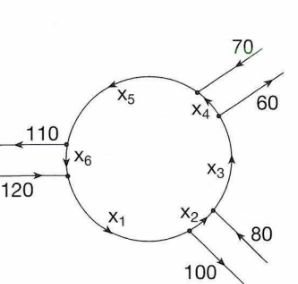
\includegraphics[width=5cm]{Strassen.png}} & \makecell[l]{Alle Winkel sind
$30\degre$ oder ein Vielfaches davon.\\
$s$ = Quadratseite = $10$ km\\
$x=\frac{s\cdot{}\sqrt{3}}{6}$ (Formel im gleichseitigen Dreieck)\\
$t = $ totale Straßenlänge\\
Senkrechte Mittelstrecke $= s-2x$\\
$t=8x+(s-2x)$\\
$t=6x+s$\\
$t=s\cdot{}\sqrt{3} + s=(1+\sqrt{3})s \approx 27.32 $ km\\
}
 \end{tabular}

Dies ist etwa 900 m kürzer, als wenn wir die beiden Diagonalen erbauen lassen.
 
\textbf{Beweis}, warum $x=\frac{s\cdot{}\sqrt{3}}{6}$ in dieser
Konstellation die beste Lösung ist:


Bezeichne $x$ die Strecke wie oben im Bild (dabei wird $s$ vereinfacht als 1
angenommen).

Bezeichne $a$ die Strecke von einer Quadratecke zur Kreuzung (in der Grafik mit
$2x$ bezeichnet; es muss jedoch noch bewiesen werden, dass $4a = 2 x$
ist).

Die totale Straßenlänge (in Abhängigkeit von $x$) wird mit $T(x)$
bezeichnet.
$$T(x) = 4a + (1 - 2x)$$

$a(x)$ kann nach dem Satz von Pythagoras berechnet werden:
$a(x) = \sqrt{\frac14 + x^2}$


Somit ist $$T(x) = 4\sqrt{\frac14+ x^2} + 1-2x$$

Beispiele: $T(0) = 3$, $T(0.5) = 2\cdot{}\sqrt{2}$

Um $T(x)$ zu minimieren leiten wir nach $x$ ab und setzten den
Ausdruck gleich Null
$$\frac{d}{dx}T(x) = 0 = \frac{8x}{\sqrt{4x^2+1}}-2$$
$$\frac{8x}{\sqrt{1+4x^2}} = 2$$
$$x = \frac1{\sqrt{12}}$$
\newpage

}%% END TRAINER



\subsection{Hungrige Kühe}\index{hungrige Kühe}\index{Kühe!hungrige}

In den folgenden Herden sind alles gleichartige Kühe, die jeden Tag dieselbe
Menge Futter fressen. Für jede Are der Wiese gilt, dass die anfängliche
vorhandene Grasmenge\index{Grasmenge} identisch ist. Ebenso wächst pro Tag und Are genau
gleich viel Gras nach.

Der Bauer hat die folgenden Messungen gemacht:

Bei 10 Aren\index{Are} fressen 10 Kühe die Wiese in 10 Tagen leer.

Bei 22 Aren fressen 15 Kühe die Wiese in 44 Tagen leer.

In wie vielen Tagen fressen nun 20 Kühe eine Wiese von 17 Aren leer?

\TNTeop{}

\TRAINER{
Es seien

$a$ die anfänglich vorhandene Grasmenge pro Are,

$n$ die täglich nachwachsende Menge pro Are,

$f$ die täglich pro Kuh abgefressene Menge.

Bei $A$ Aren, $K$ Kühen und $T$ Tagen gilt

$$A\cdot{}a + T\cdot{} a\cdot{} n - T\cdot{} K\cdot{} f = 0$$
also ergibt sich für die bekannten Messungen das folgende System
$$10a + 10\cdot{} 10n - 10\cdot{} 10\cdot{}f = 0$$
$$22a + 44\cdot{} 22n - 44\cdot{} 15\cdot{}f = 0$$

Daraus erhält man $a = 7n$ und $f = 1.7n$.

Die Anzahl Tage $T$ in der Frage erhält man nun durch Lösen der folgenden
Gleichung:

$$17a + T \cdot{}  17n - T\cdot{} 20f = 0$$
$$\Longrightarrow T = 7$$

Also fressen die 20 Kühe die 17 Aren in 7 Tagen leer.

\newpage}%% end TRAINER

\section{Professors Party}\index{Professor}\index{Party}

Der zerstreute Informatikprofessor Ph. F. aus W. lädt zusammen mit seiner Frau
zwei Paare ein. Die sechs Personen stoßen vor dem Essen mit ihren Gläsern an
oder auch nicht; dabei stoßen nicht alle mit der gleichen Anzahl Personen an. Es
hat sich herausgestellt, dass keine Frau mit Ihrem eigenen Partner angestoßen
hat. Der zerstreute Professor hat vergessen, wer denn nun mit wem angestoßen
hat, nimmt seine Frau beiseite und fragt sie: «Liebste, wer hat denn nun mit
wem alles angestoßen?»

Sie Antwortet ihm mit einem Rätsel: «Vor Dir weiß ich es nicht, jedoch haben
wir fünf anderen alle mit einer anderen Zahl von Personen angestoßen.»

Kurz darauf der Professor: «Dann ist mir alles klar. Dann haben wir zwei
nämlich genau mit denselben Personen angestoßen.»

Mit wie vielen Personen haben der Professor (und somit auch seine Frau)
angestoßen?

\TNTeop{}


\TRAINER{
\subsection{Lösungsvorschlag: Professors Party}

Eine Person hat gar nicht angestossen. Hier eine mögliche
Konstellation, wobei eine Vertauschung der Personen durchaus möglich
ist.

\bbwCenterGraphic{10cm}{AnstossenBeimProfessore.png}

\newpage}%% END TRAINRE




\section{Sehne im Kreis}\index{Sehne}\index{Kreis!Sehne}



Ein Kreis habe den Radius $r$. Diesem Kreis wird ein regelmäßiges 3-Eck
einbeschrieben (= das größtmögliche reguläre 3-Eck innerhalb des Kreises). Die Seite dieses Dreiecks
werde mit $s$ bezeichnet. Im Kreis wird eine zufällig gewählte Sehne $h$
gezeichnet.

Wie groß ist die Wahrscheinlichkeit, dass diese Sehne $h$ länger als $s$ ist?

a) Berechne $s$.\\
b) Berechne die gesuchte Wahrscheinlichkeit.

\bbwCenterGraphic{4.5cm}{Bertrand.png}

\TNTeop{}

\TRAINER{

Hierbei handelt es sich um das Paradoxon von Bertrand. Dieses Problem hat
keine «natürliche Lösung». Es hängt davon ab, was es heißt: «wird eine zufällig
gewählte Sehne $h$ gezeichnet».

Mit welchem Algorithmus soll «zufällig gezeichnet» werden?


Hier drei mögliche Lösungen wie man «zufällig gewählt» verstehen kann:


1. Gleichverteilung des Mittelpunktes der Sehne zum Mittelpunkt des
Kreises: Ist der Mittelpunkt der Sehne ($M$) näher als $\frac{r}{2}$ vom
Kreismittelpunkt entfernt, so ist die Sehne länger als
$s$. $\Longrightarrow \frac12$ aller
Sehnen sind länger als $s$.


\bbwCenterGraphic{4.5cm}{Bertrand1.png}



2.
Gleichverteilung des Mittelpunktes der Sehne innerhalb der
Kreisfläche. Nur Sehnen, deren Mittelpunkt innerhalb eines Kreises
mit Radius $\frac{r}2$ liegen, sind länger als $s$:
$\Longrightarrow \frac14$  aller Sehnen sind
länger als $s$.

\bbwCenterGraphic{4.5cm}{Bertrand2.png}


3. Gleichverteilung des Winkels zwischen Sehne und Tangente: Nur
Sehnen mit «Tangentenwinkeln» zwischen 60 und 90 Grad sind
länger als $s$. Sehnen mit Winkel zwischen 0 und 60 Grad sind
kleiner als $s$.
$\Longrightarrow \frac13 $ aller Sehnen sind länger als $s$.

\bbwCenterGraphic{4.5cm}{Bertrand3.png}

\newpage}%% END TRAINER



\section{Großvaters Problem}\index{Großvaters Problem}\index{Pfund}

Das folgende Problem aus Mathematische Rätsel und Spiele\footnote{Sam Loyd / Martin Gardner «Denksportaufgaben für kluge Köpfe», Dumont
Verlag Köln} ist weniger eine
Denksportaufgabe, als auch eine Aufgabe, die eine Recherche (z. B. Internet)
erfordert. Die Aufgabe scheint einfach, ist aber bei genauerer Betrachtung
komplex. Zu beachten gilt, dass die Aufgabe im Jahre 1978 in Deutschland
gestellt wurde.

Hier also der Originaltext der Aufgabe:

\textit{
Welches ist der Gewichtsunterschied zwischen 6
Dutzend Dutzend Pfund Federn und 1⁄2 Dutzend
Dutzend Pfund Gold?
Hier ist eines jener althergebrachten Rätsel, die immer
von einer Generation zur anderen weitergereicht
werden, ohne dass sich mal irgend jemand erdreisten
würde, die bereits feststehenden Antworten in Frage
zu stellen. Kürzlich wurde jedoch ein junger
Rätselfreund aus Bosten mit solch einem antiquierten
Juwel durch seinen Großvater konfrontiert. Und er
wartete mit einer derart ungewöhnlichen Lösung auf,
dass seinen Großeltern buchstäblich der Mund offen blieb.}

\textit{Die meisten Leute sind schon so oft gefragt worden,
welches der Gewichtsunterschied zwischen 6 Dutzend
Dutzend Pfund Federn und 1⁄2 Dutzend Dutzend Pfund
Gold wäre, dass sie über die Antwort erst gar nicht
nachzudenken brauchen. „Ein Pfund ist auf der ganzen
Welt ein Pfund“, sagen sie. «6 Dutzend Dutzend
ergeben 864 und 1⁄2 Dutzend Dutzend 72, das macht
den Unterschied von 792 Pfund aus.» }


\textit{Wenn aber die Frage in aller Ernsthaftigkeit ein
weiteres Mal gestellt wird, und wenn Sie doch noch
mal gründlich darüber nachdenken\footnote{Wie erwähnt wird reines Nachdenken nicht zur Lösung führen. Ein detailliertes
Wissen der damaligen Maße und Gewichte ist ebenso notwendig, wie eine
saubere Berechnung.} , werden Sie
entdecken, dass sie seit ihrem ersten Auftreten im
Jahre 1914 in Wirklichkeit nicht ein einziges Mal
korrekt beantwortet wurde.
}%% end TEXTIT

Tipp: Vielleicht sollte man versuchen, den Gewichtsunterschied in Gramm oder
in Unzen anzugeben!

\TNT{2.4}{}


\TRAINER{
\subsection{Lösungsvorschlag: Großvaters Problem}

Antwort Gardner: Wir müssen die Tatsache in Rechnung stellen, dass Gold
immer im Troy-System und Federn im Handelsgewicht gewogen werden. In
derlei Fällen trifft die altbewährte Maxime «Ein Pfund ist auf der ganzen Welt
ein Pfund» ausnahmsweise nicht zu.

6 Dutzend Dutzend Pfund Federn wiegen 864 Handelspfund, während 72 Pfund
Gold in Troygewicht nur 59 Pfund, 3 Unzen und 4071⁄2 Gran entsprechen. Da 864
Pfund auch als 863 Pfund, 15 Unzen und 4371⁄2 Gran bezeichnet werden können,
brauchen wir nur 59 Pfund, 3 Unzen und 4071⁄2 Gran abzuziehen, um 804 Pfund,
12 Unzen und 30 Gran zu erhalten. Das ist unsere Antwort, in
Handelsgewichtseinheiten ausgedrückt.

Der normale Bürger hat von dem Verhältnis zwischen diesen beiden Systemen
keine rechte Vorstellung. Manche glauben, das Pfund wiege bei beiden gleich
viel und sei nur bei dem einen in 16 und bei dem anderen in 12 Unzen eingeteilt.
Weit mehr Leute glauben jedoch, die Unzen seien völlig gleich, nur dass das
Handelsgewichtspfund 16 Unzen und das Troypfund 12 Unzen wiege. Keines
von beiden stimmt. Das Bindeglied zwischen den beiden Systemen, das sie
«umrechenbar» macht, besteht darin, dass ein Handelspfund 7000 Gran, ein
Troypfund dagegen nur 5760 Gran wiegt.\footnote{Im Troy-System ist 1 engl. Pfund = 12 Unzen; eine Unze = 20 Pennyweight; ein
Pennyweight = 24 Gran. – Demgegenüber ist ein Pfund im Handelsgewicht = 16
Unzen; eine Unze = 16 Dram; 1 Dram = 27.34 Gran.}

Oder in Gramm ausgedrückt:

Troy (Apotheker-)Pfund: 373.2417216g

Avoirdupois weight (Handelspfund) (USA / UK): 453.59237g

\newpage}%% end TRAINER



\section{Große Zahlen}\index{Große Zahlen}\index{Zahl!große}

Welches ist


\textit{«die kleinste natürliche Zahl\index{Zahl!natürliche}, die so groß ist, dass sie mit zweiunddreißig Silben\index{Silbe}
in Deutsch gerade nicht mehr beschreibbar ist“?}


Beispiele:

Die Zahl «zweihundert und vierundsiebzig Milliarden, achthundert und
siebenundsiebzig Millionen, neunhundert Tausend siebenhundert und
dreiundfünfzig» hat 39 Silben.

Die Zahl «zwei hoch achtunddreißig» ist zwar ähnlich groß, hat aber nur noch 6
Silben.

Die Zahl eine «Billion» (ist zwar viel größer), und hat lediglich 3 Silben.
Wir können also nicht sagen: Je größer die Zahl umso mehr Silben. Aber
vielleicht, je komplizierter zu beschreiben, desto mehr Silben.

\TNTeop{}

\TRAINER{

\subsection{Lösungsvorschlag: Große Zahlen}

So eine Zahl kann es nicht geben.

Zum Beweis nehmen wir an, es gäbe eine solche Zahl. Nennen wir diese
gefundene Zahl «Z». Dann brauche ich, um die Zahl «Z» zu beschreiben,
mindestens 33 Silben. (Sie kann ja mit 32 Silben nicht mehr beschrieben
werden.)

Die Bedingung

«die kleinste natürliche Zahl, die so groß ist, dass sie mit
zweiunddreißig Silben in Deutsch gerade nicht mehr beschreibbar ist»

benötigt
genau 32 Silben, um eine Zahl zu beschreiben. Bitte nachzählen. Nennen wir
diese eben beschriebene Zahl «X».


Ja aber, was war dann die Bedingung an «Z»? An «Z» hatten wir genau dieselbe
Bedingung gestellt wie an «X». Nämlich dass es sich um

«die kleinste natürliche Zahl, die so groß ist, dass sie mit zweiunddreißig Silben
in Deutsch gerade nicht mehr beschreibbar ist»

handelt.
Somit muss «X» gleich «Z» sein, denn beide Zahlen haben dieselbe Eigenschaft.
Um „Z“ zu beschreiben brauche ich aber mindestens 33 Silben. Daher brauche
ich (da «X» == «Z») auch für «X» mindestens 33 Silben. Wir haben aber gesehen,
dass ich «X» mit bereits 32 Silben darstellen kann, was im Widerspruch zur
Annahme steht. Somit ist unsere Annahme (es gäbe eine solche Zahl) falsch.
Natürlich können wir mit Lösungen wie

eine Milliarde hundertundeinundzwanzig Millionen, siebenundzwanzig
Tausend siebenhundertsiebenundsiebzig

(=1 121 027 777, oder 1 102 717 717

«sprich ...hundertzwei Millionen...»)


auch zufrieden sein: Wer bringt die kleinste ganze Zahl mit 33 Silben hin?
Weitere Lösungen haben sich nicht als fruchtbar erwiesen, da sie in Faktoren
zerlegt werden können, und danach als Multiplikation weniger Silben benötigen:

727 727 737 = 1613587 * 41 * 11

\newpage}%% END TRAINER
\section{Treppensteigen}\index{Treppe}
Herr F. aus W. nimmt beim Treppensteigen oft auch zwei Stufen aufs
Mal. Mehr als zwei Stufen aufs Mal hingegen nimmt er nie.

Er hat herausgefunden, dass es bei der Treppe zu Hause mit fünf Stufen
acht Varianten gibt, die Treppe mit einer seiner Varianten zu
erklimmen. Namentlich:

\begin{enumerate}
\item $1+1+1+1+1$
\item $2 + 1 + 1 + 1$
\item $1 + 2 + 1 + 1$
\item $1 + 1 + 2 + 1$
\item $1 + 1 + 1 + 2$
\item $2+2+1$
\item $2+1+2$
\item $1+2+2$
\end{enumerate}

Auf wie viele Arten kann er eine Treppe mit $n$ Stufen
($n\in\mathbb{N}$) erklimmen?
\TNTeop{%%
}%% end TNTeop
\TRAINER{\newpage
\subsection{Lösungsvorschlag}
Bei der Anzahl der Varianten die Treppe zu erklimmen, handelt es sich
um die Fibonacci-Zahlen.

Sei $A(n)$ die Anzahl der Varianten, eine Treppe mit $n$ Stufen zu
erklimmen, indem immer nur eine oder zwei Stufen aufs Mal genommen
werden.

$A(1)$ ist definitiv 1.

Ebenso kann leicht gezeigt werden, dass $A(2) = 2$; nämlich die
Varianten $1+1$ und $2$.

$A(n)$ kann aber rekursiv einfach erklärt werden. Entweder ist der
letzte Schritt eine einzelne Stufe oder der letzte Schritt ist eine
Doppelstufe.

Jede Variante der $A(n)$ Möglichkeiten kann also immer entweder so
$$... + 2$$
oder so
$$... + 1$$
aufgeschrieben werden.

Im ersten Fall bezeichnen die Punkte (...) also eine Variante aus den
Möglichkeiten, eine Treppe mit $n-2$ Stufen zu erklimmen, während beim
zweiten Fall die Punkte (...) eine der Varianten bezeichnet, bei denen
eine Treppe mit $n-1$ Stufen zu erklimmen ist.

Somit gilt
$$A(n) = A(n-2) + A(n-1).$$

Dies können wir am Beispiel von fünf Stufen einfach nachvollziehen:

Mit drei Stufen gibt es die Möglichkeiten $1+1+1$; $1+2$ und
$2+1$. Mit vier Stufen gibt es die Möglichkeiten $1+1+1+1$, $1+1+2$,
$1+2+1$, $2+1+1$ und $2+2$.
Wenn wir nun bei jeder der «Dreistufen-Möglichkeiten» hinten ein
«$+2$» ergänzen und bei jeder der «Vierstufen-Möglichkeiten» hinten
ein «$+1$» ergänzen, erhalten wir die folgenden Möglichkeiten:

$1+1+1+2$; $1+2+2$; $2+1+2$ bzw. $1+1+1+1+1$; $1+1+2+1$; $1+2+1+1$;
$2+1+1+1$; $2+2+1$.

Dies sind aber gerade genau alle Möglichkeiten, eine Treppe mit fünf
Stufen zu erklimmen.


}%% end TRAINER
\newpage
%%\bibliography{bibAll}{}\label{literatur}

\printindex

\end{document}


